\documentclass[10pt]{article}
\usepackage[margin=1in, paperwidth=8.5in, paperheight=11in]{geometry}
\usepackage{ifpdf, amsmath, amssymb, comment, color, graphicx, stmaryrd, setspace, enumitem, fancyhdr, wrapfig, textcomp, mathptmx, siunitx, multicol}
\usepackage{hyperref}
\hypersetup{
    colorlinks=true,
    urlcolor=blue,
}

\usepackage{tikz}
\usetikzlibrary{trees}

\setlength{\headheight}{14.5pt}
\newcommand{\del}{\nabla}
\newcommand{\Q}{\mathbb{Q}}
\newcommand{\R}{\mathbb{R}}
\newcommand{\Z}{\mathbb{Z}}
\newcommand{\vu}{\mathbf{u}}
\newcommand{\vv}{\mathbf{v}}
\newcommand{\vw}{\mathbf{w}}
\newcommand{\vi}{\mathbf{i}}
\newcommand{\vj}{\mathbf{j}}
\newcommand{\vk}{\mathbf{k}}
\newcommand{\vn}{\mathbf{n}}
\newcommand{\vr}{\mathbf{r}}
\newcommand{\vs}{\mathbf{s}}
\newcommand{\va}{\mathbf{a}}
\newcommand{\vF}{\mathbf{F}}
\newcommand{\vL}{\mathbf{L}}
\newcommand{\vT}{\mathbf{T}}
\newcommand{\vN}{\mathbf{N}}
\newcommand{\vB}{\mathbf{B}}
\newcommand{\comp}{\operatorname{comp}}
\newcommand{\proj}{\operatorname{proj}}
\newcommand{\orth}{\operatorname{orth}}
\newcommand\dotp[1][.5]{\,\mathbin{\vcenter{\hbox{\scalebox{#1}{$\bullet$}}}}\,}


\newenvironment{red}{\color{red}}{\ignorespacesafterend}
\newcommand{\blue}[1]{\textcolor{blue}{#1}}
\newcommand{\green}[1]{\textcolor{green}{#1}}
\renewcommand{\section}[1]{\begin{center} \textbf{#1} \\\end{center}}
%
\hyphenpenalty=5000
\setlength{\parindent}{0in}
%\oddsidemargin=-.25in
\allowdisplaybreaks
\pagestyle{fancy}
\renewcommand{\headrulewidth}{0pt}
\lhead{MATH 203}
\rhead{Fall 2024}
%\lfoot{}
%\cfoot{}

\begin{document}
%


%\onehalfspacing
\allowdisplaybreaks
%##################################################################
\section{PS\#8 -- Directional derivatives and the gradient - \red{Answer key} }

\begin{enumerate}[leftmargin=0pt]
    
    \item It's always true that the gradient points in the local direction of steepest ascent, but it's not always true that the gradient points directly at the maximum of the function. Give an example of something where the gradient doesn't point directly at the maximum. Explain why your example works. 
    
    \begin{red}
    Personally, my favorite example is Grandeur Peak, which is that mountain that's sort of at the east end of 3300 South. It has a really striking switchback ridge of exposed rock a little to the south of the peak, as you view it from the valley. I think about the gradient every time I look at that mountain. :) 
    
    Here's an overhead satellite view I grabbed from Google Maps:
    
    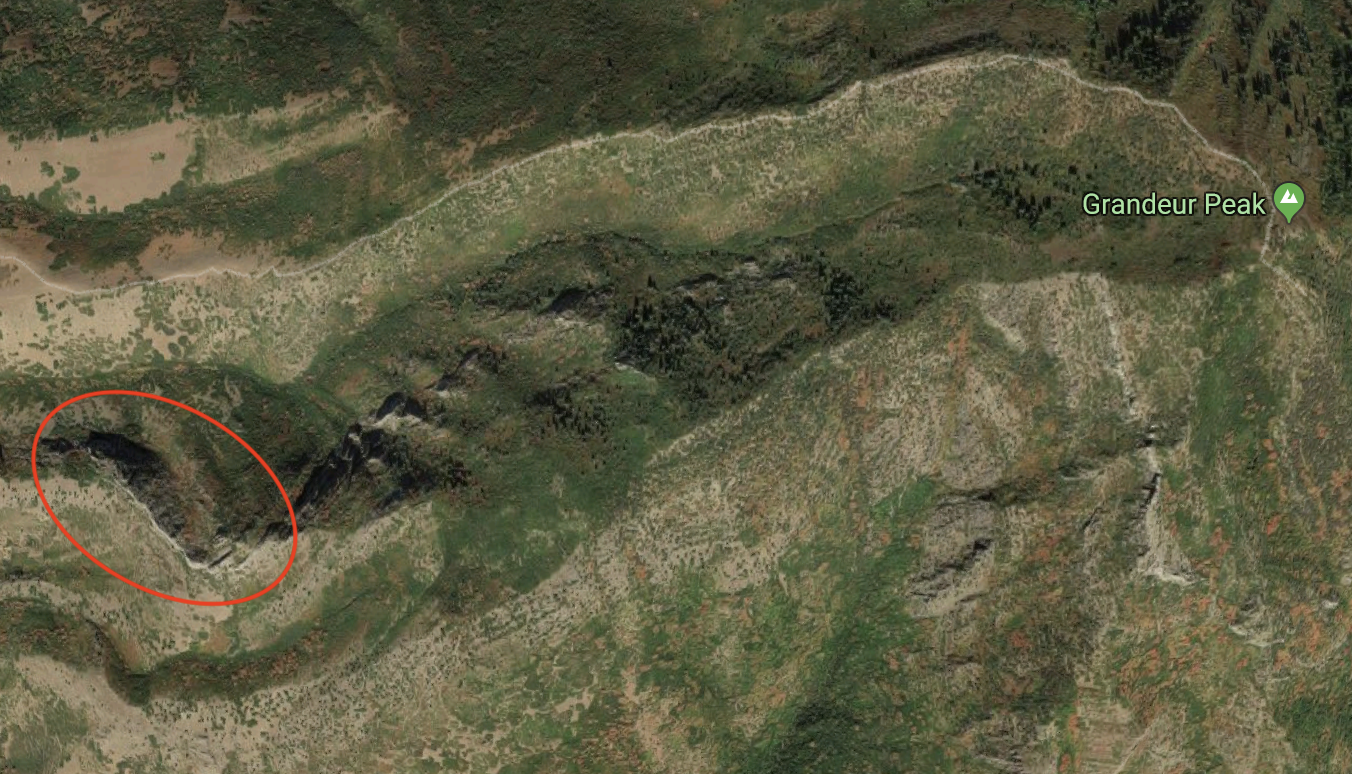
\includegraphics[width=\textwidth]{../images/grandeur.png}
    
    If you were standing directly on that ridge, the direction of steepest ascent would be along the ridge -- and the ridge points maybe $30^\circ$ or $45^\circ$ away from the peak.
    
    What's more, if you were standing in that little bowl right below the ridge, the direction of steepest ascent would be up to the top of the ridge, which is almost $180^\circ$ away from the peak!
    \end{red}
    
    \item Here's an absolutely classic problem that I think is kind of a rite of passage for students in a multivariate calculus course: the lighthouse problem.
    
    In the lighthouse at Point Gradient, the lamp has been knocked slightly out of vertical, so that the axis is tilted just a little. When the light points east, the beam of light is inclined upward at 5 degrees. When the light points north, the beam of light is inclined upward at 2 degrees.
    
    \begin{enumerate}
        \item The beam of light sweeps out a plane; let's call that plane $f(x, y)$ and say that the lighthouse is at the point $(0, 0)$ What's $f_x(0, 0)$, and what's $f_y(0, 0)$? (Hint: the answers aren't $5^\circ$ and $2^\circ$. Draw a picture and use some trigonometry to figure out the slopes.)
        
        \begin{red}
        Slope is rise over run, yeah? So $f_x(0, 0) = \tan 5^\circ$, and  $f_y(0, 0) = \tan 2^\circ$.
        
        \begin{center}
        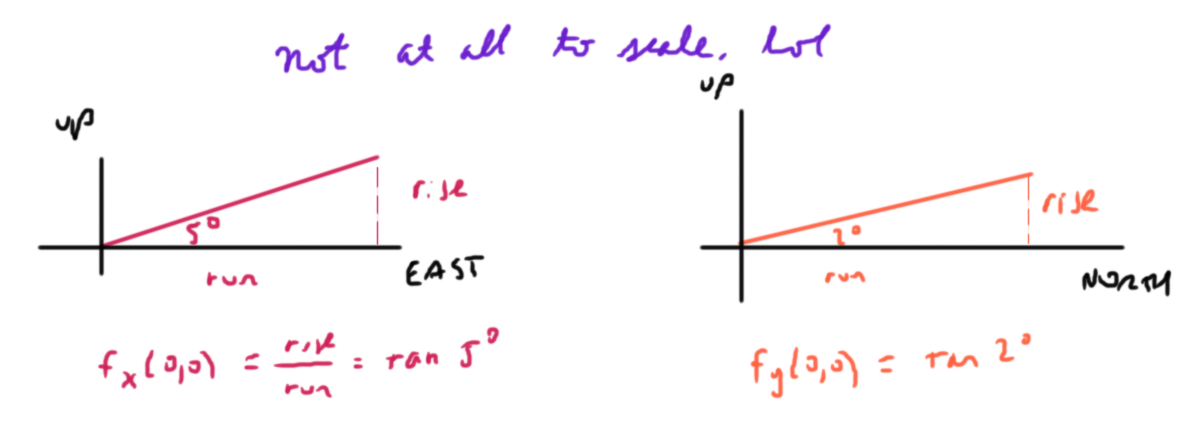
\includegraphics[width=0.5\textwidth]{../images/triangles.png}
        \end{center}
        \end{red}
        \item What's $\del f(0, 0)$? 
        
        \begin{red}
        $\del f(0, 0) = \langle f_x(0, 0), f_y(0, 0) \rangle = \langle \tan 5^\circ, \tan 2^\circ\rangle \approx \langle 0.087, 0.035\rangle$. 
        
        Note that this is a 2D vector that lives down on the map (the $xy$ plane), rather than pointing up into space.
        \end{red}
        \item Looking down from above on a map, in which direction is the light beam pointing when it's most significantly inclined from the horizontal? Explain. 
        
        \begin{red}
        My one favorite fact about the gradient is that it points in the direction of steepest slope -- in other words, most significant incline from horizontal. So, the light beam points in the direction $\del f = \langle \tan 5^\circ, \tan 2^\circ\rangle$ when it's most significantly inclined from horizontal. This is about $21.76^\circ$ north of east.
        \end{red}
        \item What is the maximum angle of elevation of the plane of the light beam from horizontal? (Hint: you'll now have to do some inverse trigonometry.) 
        
        \begin{red}
        My other favorite fact about the gradient is that its magnitude is the value of the steepest slope. In our case, $|\del f| = \sqrt{(\tan 5^\circ)^2 + (\tan 2^\circ)^2} \approx \sqrt{0.0089} \approx 0.0942.$ This is our rise over run: the plane of the beam of light is inclined by this amount from horizontal when it points in the direction of $\del f$. So if we were to draw a triangle again, we'd have a rise of 0.0942 and a run of 1, which means that our angle is $\arctan(0.0942) \approx 5.381^\circ.$
        \end{red}
        \item Do you think we should be worried about this amount of tilt? I'd hate to have a ship out there that isn't able to see the lighthouse because the beam is shooting too high.
        
        \begin{red}
        (Your answer to this question might vary!) Let's say that at minimum, someone standing on board a ship is, like, 10 feet off the water. Some quick trig tells me that if a ship is more than $\dfrac{10}{\tan(5.381^\circ)} \approx 106$ feet away from the shore, the light beam could be going over their head to where they couldn't see it. Dang, that seems pretty close. I'm worried about this and I'm putting in for a repair order.
        \end{red}
    \end{enumerate}
    
    \end{enumerate}

\end{document}